\documentclass[12pt]{article}
\usepackage[a4paper, margin=2cm]{geometry}
\usepackage{titlesec}
\usepackage{setspace}
\usepackage{amsmath}

% for tables
\usepackage{array}
\usepackage{booktabs}

% package that forces LaTeX to place an image in the exact position as it determied in the code
\usepackage{float} 

% for a rectangular box
\usepackage[most]{tcolorbox}

% package for multiple columns
\usepackage{multicol}
\setlength{\columnsep}{0.8cm} % separation between columns

\usepackage[utf8]{inputenc}

\usepackage{graphicx}
\usepackage{xcolor}

% For rotating figures, tables, etc. including their captions
\usepackage{rotating}

% small font size in the captions
\usepackage[font=small]{caption}

% header
\usepackage{fancyhdr}
\setlength{\headheight}{15.0pt}
\usepackage{ifthen}
\pagestyle{fancy}
\fancyhf{}
\fancyhead[L]{\ifthenelse{\value{page}=1}{}{Lessons \& Tutorials in Theoretical Chemistry}}
\fancyhead[R]{\ifthenelse{\value{page}=1}{}{Homework}}
\fancyfoot[C]{\thepage}

% bibliography
\usepackage[numbers]{natbib}
\bibliographystyle{unsrtnat}
\usepackage[colorlinks=true, linkcolor=blue, citecolor=blue, urlcolor=blue]{hyperref}
\renewcommand{\bibfont}{\small} % small font in the bibliography

% For DOIs in references
\usepackage{doi}
\renewcommand{\doitext}{DOI: }

% For code snippets
\usepackage{listings}

\definecolor{codegreen}{rgb}{0,0.6,0}
\definecolor{codegray}{rgb}{0.5,0.5,0.5}
\definecolor{codepurple}{rgb}{0.58,0,0.82}
\definecolor{backcolour}{rgb}{0.93,0.93,0.93}

\lstdefinestyle{mystyle}{
    backgroundcolor=\color{backcolour},   
    commentstyle=\color{codegreen},
    keywordstyle=\color{magenta},
    numberstyle=\tiny\color{codegray},
    stringstyle=\color{codepurple},
    basicstyle=\ttfamily\footnotesize,
    breakatwhitespace=false,         
    breaklines=true,                 
    captionpos=b,                    
    keepspaces=true,                 
    numbers=left,                    
    numbersep=5pt,                  
    showspaces=false,                
    showstringspaces=false,
    showtabs=false,                  
    tabsize=2
}
\lstset{style=mystyle}


\title{Quantum Dynamics - Homework}
\author{Albert Makhmudov}
\date{19/03/2025}

\begin{document}

\maketitle

\section*{Data Availability}
The source code of this project as well as the example input files are available at the corresponding \href{https://github.com/almakhmudov/LTTC-Homework--QD}{Github page}. There one could also find the example output files and the detailed instructions on how to run and compile the code. The example output files are \texttt{gif} animations of the wavepacket propagation that complement the results in \autoref{fig:snapshots}. The source code of this project is written in \texttt{Fortran90}, whilst the figures were generated using \texttt{gnuplot}.

\section*{Code Overview}

\subsection*{Input}
In order to run the code, one should provide two input files, namely \texttt{wavepacket} and \texttt{potential}. It's important to name the files this way. \\

The \texttt{wavepacket} file should contain the following parameters: number of lattice points, initial position of the wavepacket, the initial width, propagation time step, total number of steps, snapshot frequency, total number of coefficients and the coefficients themselves. \\

The \texttt{potential} file should specify the type of a potential, e.g. harmonic and double well are supported, as well as the angular frequency in case of the harmonic potential and the barrier height in case of the double well potential. In both input files, each parameter should be written on a separate line. The example input files can be found in \texttt{harmonic/wavepacket} and \texttt{harmonic/potential}, respectively. \\

\subsection*{Wavepacket Initialisation and Normalisation}
In this project, instead of using a gaussian wavepacket, the wavepacket is initialised as a superposition of the eigenstates of the harmonic oscillator. At $t = 0$, the wavepacket is given by the following expression:
\begin{equation}
    \Psi(x, t = 0) = \sum_{n=0}^{\infty} c_n \Phi_n(x)
\label{eq:wavepacket}
\end{equation}

Where the eigenstates of the quantum harmonic oscillator are calculated according to the following formula:
\begin{equation}
    \Phi_n(x) = \frac{1}{\sqrt{2^n n!}} \left( \frac{m\omega}{\pi} \right)^{1/4} e^{-m\omega x^2 /2} H_n(x\sqrt{m\omega})
    \quad (n = 0,1,2, \cdots)
\label{eq:eigenstates}
\end{equation}

$H_n$ is the Hermite polynomial of order $n$. We'll touch upon the implementation of the Hermite polynomials in the next section. While initialising the wavepacket according to the \autoref{eq:wavepacket} and \autoref{eq:eigenstates} as shown in \autoref{lst:initpsi}, the calculation of a norm of the wavepacket is performed alongside. The code snippets for the wavepacket initialisation are provided below. \\
    
\begin{lstlisting}[language=Fortran, firstnumber=104, label={lst:initpsi}, caption=Initialisation of the wavepacket in the \texttt{initpsi} subroutine.]
norm = 0.0d0                                                            
nmax = size(coeff) - 1                                                  
do i = -npoints/2 + 1, npoints/2                                       
    x = dble(i) * dx
    if (i > 0) then
        j = i
    else     
        j = i + npoints
    endif
    psi0(j) = 0.0d0                                                
    do n = 0, nmax                                                   
        call factorial(n, fact)                                   
        psi0(j) = psi0(j) + &                                   
                coeff(n+1) * &
                (1.0d0 / sqrt(2.0d0**n * fact)) * &
                (mass * angfreq / pi)**0.25d0 * &
                exp(-mass * angfreq * alpha * (x-x0)**2.0d0 / 2.0d0) * &
                hermite(n, (x-x0) * sqrt(mass * angfreq)) 
    end do
    norm = norm + abs(psi0(j))**2.0d0 * dx                        
end do
\end{lstlisting}

As soon as the norm of the wavepacket is calculated, the wavepacket is normalised as shown in \autoref{lst:normalisation}. The normalisation is performed by dividing each element of the wavepacket by the square root of the norm. This ensures that the wavepacket is properly normalised. \\

\begin{lstlisting}[language=Fortran, firstnumber=126, label={lst:normalisation}, caption=Normalisation of the wavepacket in the \texttt{initpsi} subroutine.]
norm = 1.0d0 / sqrt(norm)                                              
do i = -npoints/2 + 1, npoints/2
    x = dble(i) * dx
    if (i > 0) then
        j = i
    else     
        j = i + npoints
    endif
    psi0(j) = norm * psi0(j)                                         
end do 
\end{lstlisting}

Due to the need of computing the factorials, the corresponding subroutine is implemented as shown in \autoref{lst:factorial}. The factorial is calculated up to the $n$th order. \\

\begin{lstlisting}[language=Fortran, firstnumber=148, label={lst:factorial}, caption=Calculation of the factorial up to the $n$th order in the \texttt{factorial} subroutine.]
    result = 1.0d0
    do i = 1, n                                                            
       result = result * i
    end do
\end{lstlisting}

\subsection*{Hermite Polynomials}
The Hermite polynomials are calculated using the following recurrence relation:
\begin{equation}
    H_n(y) = 2y H_{n-1}(y) - 2(n-1)H_{n-2}(y)
    \quad \left( H_0(y) = 1, \, H_1(y) = 2y \right)
\end{equation}

Where $H_0$ isn't calculated explicitly. The reason to use Hermite polynomials in the wavepacket initialisation is due to the fact that the eigenstates of the quantum harmonic oscillator are expressed in terms of the Hermite polynomials as shown in \autoref{eq:eigenstates}. Specifically, the physicist's Hermite polynomials are used in this project. The code snippet for the calculation of the Hermite polynomials is provided in \autoref{lst:hermite}. \\

\begin{lstlisting}[language=Fortran, firstnumber=166, label={lst:hermite}, caption=Calculation of the Hermite polynomials up to the $n$th order in the \texttt{hermite} function.]
if (n == 0) then                                                       
Hn = 1.0d0
elseif (n == 1) then                                                
Hn = 2.0d0 * y
else                                                                 
H0 = 1.0d0
H1 = 2.0d0 * y
do i = 2, n                                                         
   H_prev = H1
   H1 = 2.0d0 * y * H1 - 2.0d0 * (i - 1) * H0                       
   H0 = H_prev
end do
Hn = H1
endif
\end{lstlisting}

\section*{Results and Discussion}
The wavepackets were propagated a the bottom of the harmonic potential with the angular frequency $\omega = 0.2825$ fs$^{-1}$. More over they were propagated for 5000 steps with a 0.1 fs time step. The initial width of the wave packet was equal to 1.0 Bohr$^{-2}$ and the snapshots were taken each 10th step. The wavepackets were propagated with different number of eigenstates, namely 1, 2, 3, and 5. The time evolution of the wavepackets is shown in \autoref{fig:snapshots}. \\

The wavepackets with a single eigenstate are stationary, whilst the wavepackets with multiple eigenstates are oscillating. The oscillations are due to the fact that the wavepacket is a superposition of the eigenstates of the harmonic oscillator. The more eigenstates are included in the wavepacket, the more oscillations are observed. The wavepacket with 5 eigenstates oscillates the most. The oscillations are periodic and the period of the probability density is calculated below. \\

The period of the probability density for the harmonic oscillator case can be calculated from the angular frequency as follows:
\begin{equation}
    T = \frac{2\pi}{\omega}
\label{eq:period}
\end{equation}
Therefore the periods $T$ of the corresponding probability densities are equal to $22.23$ fs. \\

Speaking of the symmetry, the wavepackets with the even number of eigenstates have symmetric probability densities of the wavefunction. On the other hand, the odd number of eigenstates results in the probability densities being assymetric as can be seen in \autoref{fig:snapshots}. \\

\begin{sidewaysfigure}[ht!]
    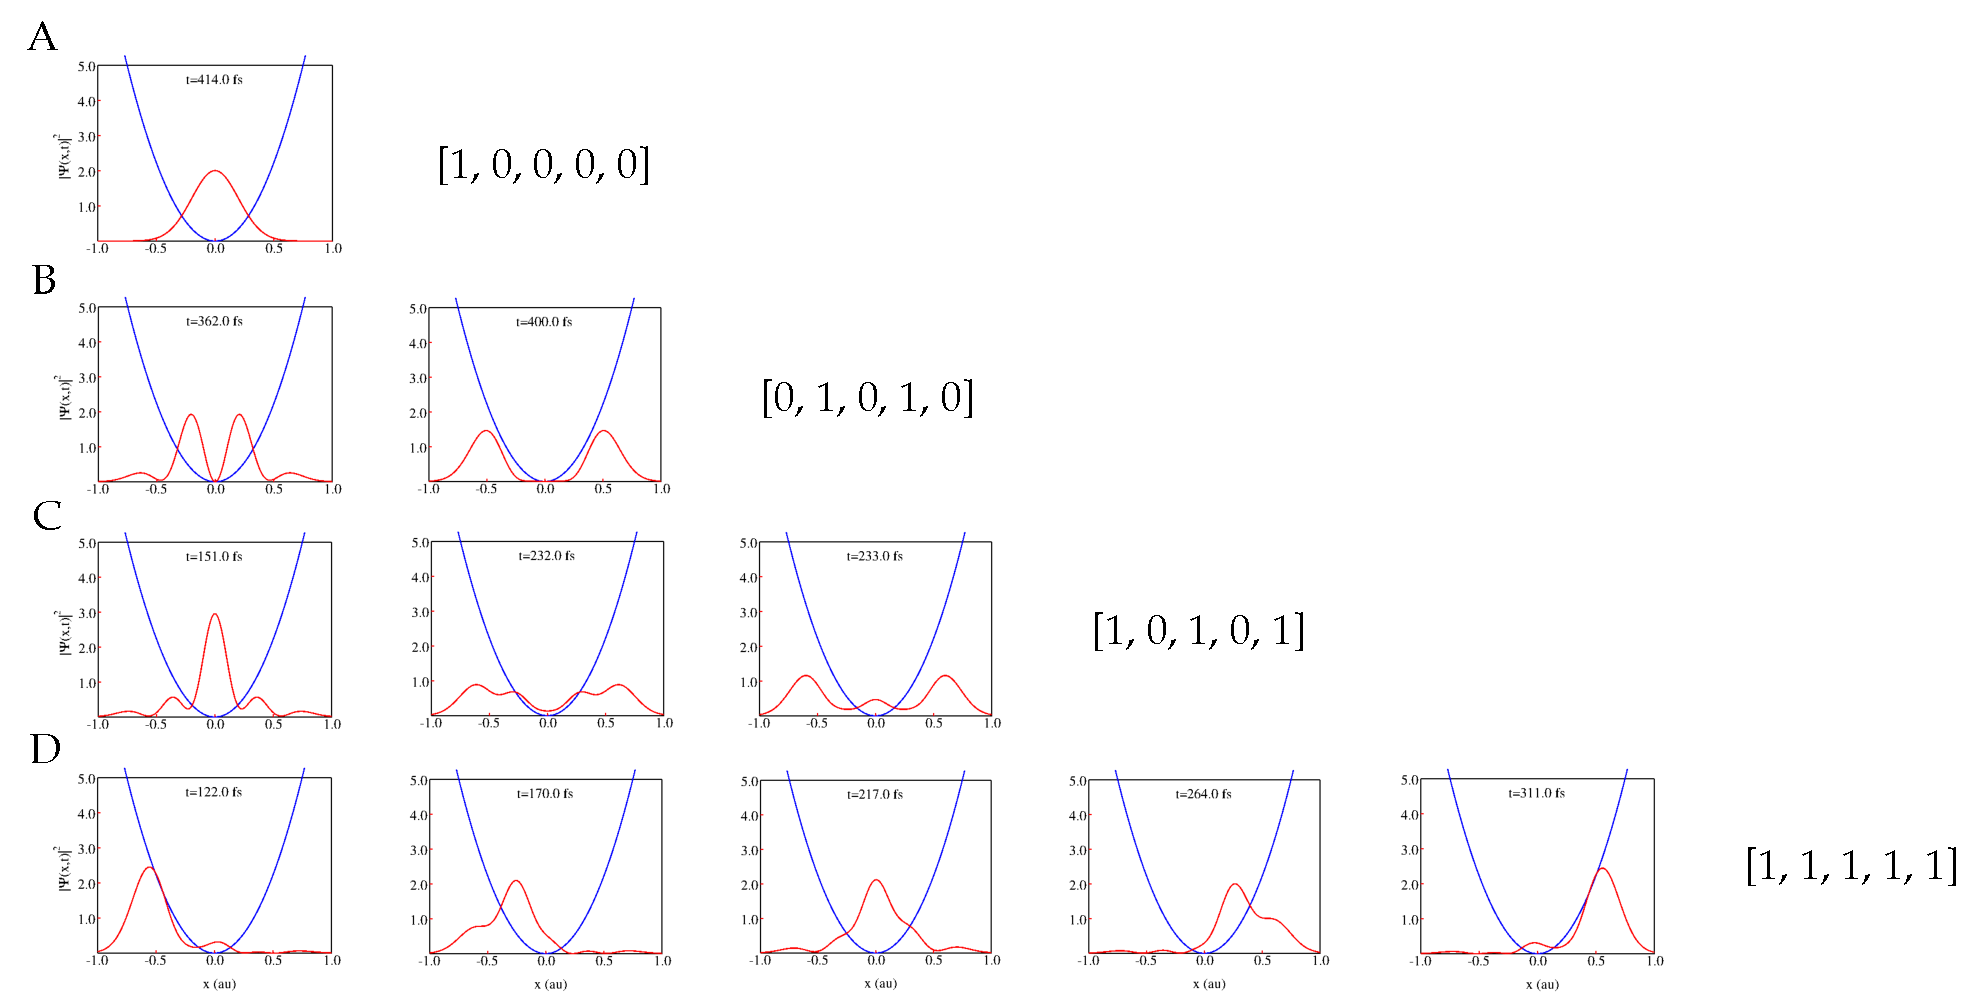
\includegraphics[width=\textwidth]{snapshots.pdf}
    \caption{Time evolution of the wavepackets with different number of eigenstates. The wavepackets were propagated using the \textbf{(A)} $[1, 0, 0, 0, 0]$, \textbf{(B)} $[0, 1, 0, 1, 0]$, \textbf{(C)} $[1, 0, 1, 0, 1]$, and \textbf{(D)} $[1, 1, 1, 1, 1]$ coefficients.}
    \label{fig:snapshots}
\end{sidewaysfigure}
\clearpage

The underlying reason for this is the wavefunction itself. The soutions alternate between even and odd functions around the $x = 0$ resulting in different symmetries of the probability densities \citep{quant_harmonic_osc}. \\

While the particle with one eigenstate spends the majority of time at the bottom of the potential, the particles with multiple eigenstates oscillate. The chance of finding the particle outside of the potential increases as well. For instance, for a particle with one eigenstate this probability is around 16 \% \citep{the_quant_harmonic_osc}. \\

\section*{Generative AI Usage}
In this work, \href{https://chatgpt.com}{ChatGPT} large language model was used to check grammar and spelling of the main body of text, whilst \href{https://www.perplexity.ai}{Perplexity} was utilised for the sake of literature search.

\section*{Acknowledgments}
This project is based on data and instructions provided by Arjan Berger available at the aforementioned \href{https://github.com/almakhmudov/LTTC-Homework--QD}{Github page}.

\bibliography{references}

\end{document}